\documentclass[9pt,twoside,lineno]{pnas-new}
% Use the lineno option to display guide line numbers if required.

\templatetype{pnassupportinginfo}

\title{Water resource utilization regimes at a basin scale: transition framework and development traps}
\author{Shuang Song, Shuai Wang, Bojie Fu, Xutong Wu (complete author list)}
\correspondingauthor{Shuai Wang.\\E-mail: shuaiwang@bnu.edu.cn}

\begin{document}

%% Comment out or remove this line before generating final copy for submission; this will also remove the warning re: "Consecutive odd pages found".
% \instructionspage

\maketitle

%% Adds the main heading for the SI text. Comment out this line if you do not have any supporting information text.
\SItext{This supplementary document consists of four \textit{Methods} sections, 9 \textit{SI Appendix} figures and 2 \textit{SI Appendix} tables. Firstly, we introduced our study area, the Yellow River Basin, and its subdivisions in the section Methods S1. Then, we give a detailed description of used datasets and analysis their uncertainties in the section Methods S2. Further, we introduced how to harmonized different datasets with various spatial and temporal scales in Methods S3. Finally, the index along with corresponding indicators are introduced in the section Methods S4.}


% \subsection*{Brief description of Supplementary Information contents: }
% Type or paste text here. This should be additional explanatory text such as an extended technical description of results, full details of mathematical models, etc.   

% tag 研究区定义
\newpage
\section*{Methods S1. Definition of study area}

\subsection*{Region divisions of Yellow River Basin}

The study area is the Yellow River Basin (YRB, see Fig. S1-A), which had experienced the most intense water exploitation and the most dramatic shifts of management regime in China. 
According to the Yellow River Conservancy Commission (YRCC), an administrative government directly under the Ministry of Water Resources at the basin level, the upper, middle and lower reaches of the Yellow River can be distinguished by the characteristic of river. 
However, there is another scheme suggesting that the upstream only refers to river source areas with little human disturbance and high water retention capacity.
% TODO 这里补充参考文献,黄河上游的划分争议 
Anyhow, since the socio-economic and natural conditions were both considered in this study, we integrated the two schemes above and divided the Yellow River Basin into four regions, which can be distinguished by three important hydrological control stations (see Fig. S1-B). 
Previous studies have also shown that such a division is valid when both social water use and the natural conditions of the basin are considered, as the regions exhibit strong heterogeneity among themselves (see Fig. S1-C) \cite{wangYellowRiverWater2019}:

\begin{itemize}
    \item \textbf{Source Region (SR):} Over 50\% of natural runoff was produced in this region. The most ecology function here is water conservation, as sparsely populated and less economically developed.
    \item \textbf{Upper Region (UR):} With the highest per capita irrigated land area, there are numbers of large irrigation lands in this region. However, because of backward production methods, efficiency of irrigation are used to be very low.
    \item \textbf{Middle Region (MR):} Crossing Loess Plateau, famous rich-sand area, Yellow River loads most of its sediments here with the highest soil erosion risk. To reverse this situation, the grain for green project changed the water utilization here strikingly.
    \item \textbf{Lower Region (LR):} With dense population and the traditional agricultural trajectory, lower region used to be the largest water use region. However, as the industrial transformation going, proportion of agriculture keeps decreasing, but LR is still the largest water use region in each aspect.
\end{itemize}

In general, there are inter-regional differences in the economic layout, distribution of water resources, distribution of water consumption, and population distribution of the Yellow River Basin (see Fig. S2). On the basis of these fundamental differences, social development and watershed management continue to influence and reshape their changes, making the Yellow River Basin the world's most intimately connected and dramatically changing large river basin. Thus, as a case study for analysing the evolution of the human-water relationship, it possesses typicality.

% \subsection*{Importance of water resource to society within the YRB}
Water resources make an irreplaceable contribution to the development of society in the YRB. Firstly, each aspect of economic development highly depended on water resources, since the most water use patterns are positively correlated with the region's key economic indicators (see Fig. S2-A, B and D). 
% Secondly, their relationships have noticeably changed over the study period. In particular, the major water-consuming sectors have undergone particularly dramatic changes (see Fig. S3-B). 

% 举农业案例作为说明
%For an example, the agriculture, which occupied over 60\% of water consumptions, whose relationship with regional economic development has weakened, and there have been significant changes in water consumption per unit and total water consumption (see Fig. S).

\subsection*{Changes brought from human activities on the YRB}
Humans are constantly modifying the water cycle processes in the watersheds as society develops.
\begin{itemize}
    \item Firstly, the YRB has been subject to strong intervention by human activities since ancient times, while the last 60 years have seen the most dramatic changes. Under human influence, the Yellow River's surface runoff, sediment transport, and human water consumption patterns have all undergone multiple regime shifts in the last 60 years
    % \cite{}.
    % TODO 这里增加参考文献,黄河近六十年的变化 
    \item Secondly, landscapes in the YRB have significantly altered by human activities, which can both change the natural and the social water cycle. For an example, “grain for green” project has produced a significant change of landscapes in the middle region (MR) of YRB. With the addition forest in an erosion-prone area, water use patterns in the area and surface runoff patterns in the middle and lower reaches have been radically altered.
    % TODO 这里增加参考文献  景观的变化 \cite{}
    \item Thirdly, a series of management practices have promoted in order to govern the YRB. Since the establishment of the Yellow River Water Conservancy Commission in XX, the agency has continued to reform and expand, eventually forming a basin management agency with unified coordination, scheduling and regulatory functions. Since the promulgation of the Water Law in xxx, the Ministry of Water Resources, the YRCC and other relevant agencies have issued a series of policies to carry out comprehensive river basin management under the guidance of national laws (see \textit{SI Appendix} Table S2).
\end{itemize}
Historic and recent river basin management practices have strong impacts on water utilization.


% tag 数据集介绍
\newpage
\section*{Methods S2. Detailed information on datasets}

Multiple types of dataset were used in this study (see Table S1). 
\subsection*{Statistical datasets}
% 使用了GDP数据,年鉴数据,还有从第二次水资源调查提取的数据
For statistics, we used GDP data, water resources uses data extracted from the 2nd National Water Resources Assessment Program \cite{zhouDecelerationChinaHuman2020} and statistical yearbook data of YRB. GDP data from the China Macro data in the Wind database, which firstly aggregated from annual reports of the provinces. Water resources use dataset was published by Zhou et al. \cite{zhouDecelerationChinaHuman2020}, which records water utilization in different sectors along with social-economic situations in perfects level. This dataset was mainly extracted by 2nd National Water Resources Assessment Program launched in 2002, led by the National Development and Reform Commission and the Ministry of Water Resources (see ref (1) and \url{http://www.mwr.gov.cn/english/publs/} for more details). Since then, the statistics from the survey using the same criteria have been supplemented and harmonized to the 2013 administrative divisions. 
%TODO xx 这里把每个数据的子类介绍清楚
The data covers a total of subcategories of water use under four broad categories: agriculture, industry, urban and rural, but does not distinguish between surface water and groundwater. There is uncertainty at the county scale for each disaggregated water use sector, but because the data are corrected for statistical information using the water balance method, the data are adequate for the regional scale and the four broad water use categories used in this study.
Finally, in order to make a simple distinction between the proportion of surface water and groundwater extraction where needed, we use basin-scale water resources annual reporting data. Yearbook data of YRB documenting surface water resources and groundwater resource extraction in each watershed and province. 


\subsection*{Hydrological datasets}
For hydrological datasets, reservoirs data and a measured runoff data were used in this study.
The reservoir dataset were collected by Wang et al. \cite{wangYellowRiverWater2019}, which introduced includes the major new reservoirs built in the Yellow River Basin since 1949. Of these, we consider the reservoirs marked as pivot projects by the YRCC to be more important, as they are directly involved in water resources management in the basin (\url{http://www.yrcc.gov.cn/hhyl/sngc/}). Annual runoff data derived from hydrological station measurements.

\subsection*{Political datasets}
%对于政策数据集,我们选取了《黄河流域综合规划》中流域级部门(如黄河水利委员会)级以上(如国家部委)颁布施行的与黄河流域有关的法律政策。此外,我们还从《黄河水利委员会组织沿革》一书中获取的黄河水利委员会作为黄河流域级管理单位的组织沿革情况,以反映流域级管理举措的实施情况。
For the policy data set, we select the laws and policies related to the Yellow River basin promulgated and implemented by departments at and above the river Basin level (such as Yellow River Conservancy Commission) in the Comprehensive Planning for the Yellow River Basin (such as national ministries and commissions) \cite{yellowriverconservancycommissionYellowRiverBasin2013}. In addition, we also obtain the organizational evolution of the Yellow River Water Conservancy Commission as a watershed management unit from the book Organizational Evolution of the Yellow River Water Conservancy Commission to reflect the implementation of watershed management measures \cite{yellowriverarchivesOrganizationalHistoryYellow2004}.


% tag 数据处理
\newpage
\section*{Methods S3. Harmonization of datasets}
% TODO 这里要强调省级数据和县级数据在不确定性上的差异
% 由于我们的数据集来源广泛,且具有不同的空间尺度,我们需要在区域尺度(SR,UR,MR和DR)上对数据进行调和,根据数据的空间尺度有不同的处理方式。
Due to the wide sources of our data set and the different spatial scales, we need to reconcile the data on the regional scale (SR, UR, MR and DR), and have different processing methods according to the spatial scale of the data.
\begin{itemize}
    \item 1. Watersheds:
    % 由于流域的分区由水文分区决定,所以水文年报数据和实测径流量数据都能直接根据其对应的水文站直接划分。
        Due to the fact that the subdivision of a basin is determined by hydrological subdivision, hydrological annual data and measured runoff data can be directly divided according to their corresponding hydrological stations.
    \item 2. Perfects:
    % 在市县尺度下,我们分别计算了市县在不同流域分区中所占的面积,选取其中最大的区域,如果该面积占该县面积的95%以上,则认为该市属于该区域,即:
        At the scale of cities and counties, we respectively calculate the area occupied by cities and counties in different watershed districts, and select the largest region. If this area accounts for more than 95\% of the area of the county, the city is considered to belong to this region, that is:
        $$ S_{ij} = MAX(S_ij / S_i)$$
        where $i$ refers a certain perfect and $j$ refers a region within YRB, i.e. SR, UR, MR, or DR. $S_i$ refers the area of perfect $i$, and $S_{ij}$ refers intersecting area between perfect $i$ and region $j$.
        We define perfect $i$ belongs to region $j$ if their intersecting area over 95\% of $S_i$, i.e.:
        $$ MAX(S_{ij}) > 0.95 * S_i $$
    \item 3. Province:
    % 在省域尺度的数据(即不同行业的GDP数据)更多用以定性描述,且不与县域尺度数据进行横向比例,因此数据的精度不再重要。我们采用了粗略的处理。即,根据不同区域包含的主要省份,判断该省的数据被融合进哪个区域。参考传统划分惯例,我们进行的划分是:
    Data at the provincial scale (i.e., GDP data of different industries) are more used for qualitative description, and do not carry out horizontal proportion with data at the county scale, so the accuracy of the data is no longer important. We have adopted a rough treatment. That is, according to the major provinces contained in different regions, determine which region the data of that province is merged into. Referring to the traditional division practice, we made the following division:
    \begin{itemize}
        \item SR: Qinghai Gansu and Sichuan,
        \item UR: Ningxia and Neimeng,
        \item MR: Shanxi and Shaanxi,
        \item DR: Shandong, Hebei and Henan.
    \end{itemize}
\end{itemize}

% 最后,当我们处理位置点数据(如水库修建位置数据时),根据其所在位置判断其所属省份,再按照省尺度的区域归类方式进行处理。经过上述处理,所有的数据都能很好的在区域尺度得到协调。
Finally, when we process the location data (such as the location data of reservoir construction), we judge the province it belongs to according to its location, and then process it according to the regional classification method on the provincial scale. After the above processing, all the data can be well coordinated at the regional scale.

\newpage
% 指数介绍
\section*{Methods S4. Water Utility Regime Index}
% 水资源利用稳态指数考虑了流域尺度内人类利用水资源时最主要的三个维度,分别对应了 “有多少水”,“怎么用”和“给谁用”三个问题。
The steady-state index of water resources utilization considers the three most important dimensions of human utilization of water resources at the watershed scale, corresponding to the three questions of ``how much water'', ``how to use'' and ``for whom, for where'' respectively. 
% TODO 这里需要增加参考文献,证明这三个维度是最重要的。
% 无论如何,为了让这些维度能够被量化,我们寻找或发明了共计三个度量指标来对应指示其变化趋势:
In order for these dimensions to be quantified, we found or invented a total of three metrics corresponding to the trend indicating their change: SFV Index, Non-provisioning Share and Allocation Entropy Metric.

\subsection*{Stress: SFV-index}
	%* 提出了很多的指标度量水压力,如水资源压力指数,水资源xxx等
	There is how much water can be used in a certain basin? How many stresses has societies put on the water resources of the basin? Various metrics, therefore, proposed for water stress (e.g. water scarcity, water stresses index, scarcity-flexibility-variability index), where the dimensions of human impact are increasingly valued.
	%* 其中SFV指数比较有用
    Among of them, by taking changes of water flexibility and variability into account,	the scarcity-flexibility-variability (SFV) index focus more on dynamic responses to water resources in developing perspective, which considered a valid metric of temporal changes in water stresses \cite{qinFlexibilityIntensityGlobal2019}.
    %* 该指标从人类开发利用水资源的角度,考虑了影响人类感知水资源压力的三个方面:水资源的总量、水资源变异性、人类利用水资源的灵活性。
    
	To apply this method, we need to combine three metrics following: 
	
	First for scarcity, $A_{i, j}$ is the total water consumption as a proportion of regional multi-year average runoff volume, in year $j$ and region $i$:
	$$ A_{i, j} = \frac{WU_{i,j}}{R_{i, avg}} $$
	Second for flexibility, $B_{i, j}$ is the inflexible water use $WU_{inflexible}$ (i.e. for thermal power plants or humans and livestock) as a proportion of average multi-year runoff, in year $i$ and region $j$:
	$$ B_{i, j} = \frac{WU_{inflexible}}{R_{i, avg}} $$
	Finally for variability, the capacity of the reservoir and the positive effects of storage on natural runoff fluctuations are also considered.
	$$ C_i = C1_i * (1 - C2_i) $$
	$$ C1_{i, j} = \frac{R_{i, std}}{R_{i, avg}} $$
	$$ C2_{i} = \frac{RC_{i}}{R_{i, avg}}, \ if RC < R_{i, avg} $$
	$$ C2_{i} = 1, \ if RC >= R_{i, avg} $$
	In all the equations above, $R_{i, avg}$ is the average runoff in region $i$, $RC_i$ is the total storage capacities of reservoirs in the region $i$, $R_{i, std}$ is the standard deviation of runoff in the region $i$.

	Finally, assuming three metrics (scarcity, flexibility and variability) have the same weights, we can calculate $SFV$ index after normalizing them:
	$$ V = \frac{A_{normalize} + B_{normalize} + C_{normalize}}{3} $$
	$$ a = \frac{1}{V_{max} - V_{min}}; $$
	$$ b = \frac{1}{V_{min} - V_{max}} * V_{min} $$
	$$ SFV = a * V + b $$

\subsection*{Priority: Non-provisioning share}
    %* 从消耗水 到 利用水
    % xxx等人通过考虑消费品中的水消耗提出了虚拟水理论,发现水资源作为粮食与消耗产品的供给是水资源的主要用途,且能够随着贸易发生流动。但随着水资源利用方式的变迁,在其基础上兴起的水足迹研究,则进一步泛化了水相关的产品和服务概念。如今,世界非产品形式供给于人类的水资源已达xx%,范围包含了xxxxxx等方式,人类社会发生着从“消耗水”向“利用水”的倾斜。
    How to use water resources? There has been put forward the virtual water theory by considering the water consumption in consumer goods, and found that the supply of water resources as food and consumption provisions is the main use of water resources, and can flow with trade. However, with the change of water resource utilization mode, the water footprint research on the basis of water footprint further generalizes the concept of water-related provisions and services. Today, the world's non-provisioning form of water supply to human beings are increasing more than 20 times faster growth, including industry, services and other ways, the human society is occurring from ``consumption of water'' to ``use of water'' tilt.
    % TODO 这里要补充一些材料
    % *这里我们使用非用于供给性的水资源量所占的比例作为指标,即:
    Here, we use Non-Provisioning Shares (NPS) of used water resources as a metric to indicate priority of water utility:
    $$ NPS_{ij} = \frac{WU_{indirect, i, j}}{WU_{direct, i, j} + WU_{undirect, i, j}} $$
    where $i$ refers a certain year and $j$ refers a certain region. Thus, $WU_{i,j}$ means the water use in $i$ year and region $j$, where $direct$ part and $undirect$ part indicate provisioning sectors and non-provisioning sectors respectively.
    %* 直接用水和非直接用水
    % 在本研究中,我们将牲畜用水、农村或城市的居民用水、农业用水认为是供给型用水。对应的,非供给性用水常常是工业用水,其中以能源用水为主。根据广泛的研究表明,水-粮食-能源之间存在广泛的联结,是水资源供应倾向性的一种体现,其中供给性用水常常是能够作为支持农产品生产的关键,而非供给水则更多参与了工业等社会过程。对中国整体而言,如果只考虑农业生产,中国是虚拟水贸易的流入国。但如果考虑工业耗水,中国则向外出口虚拟水资源。而黄河作为水资源高度稀缺的流域,更需要考虑两者之间的权衡,因此采用该比例作为指标能够简单、直接、有效地反映用水 priority 的变化。
    % TODO 这里要补充一些材料 Li 2020,虚拟水贸易,水粮食能源的联结
    In this study, we consider water for livestock, water for rural or urban residents and water for agriculture as provisioning water. Correspondingly, non-provisioning water is often industrial water, mainly energy water. Extensive studies have shown that there is a wide connection between water, food and energy, which is a manifestation of water supply tendency, in which provisioning water is often the key to support the production of agricultural products, while non-provisioning water is more involved in industrial and other social processes. For China as a whole, if only agricultural production is considered, China is the recipient country of virtual water trade. But if industrial consumption is taken into account, China is exporting virtual water. However, as a river basin with high degree of water resource scarcity, the trade-off between the two has always been treated with greater value; thus, the adoption of this ratio as an indicator can simply, directly and effectively reflect the change of priority with water.

\subsection*{Configuration: Allocation Entropy Metric}
    %* 哪里利用水资源?  
    Where to use water resources? 
    % * 设计了一个熵指标
    % 水资源的分配一直是难题,需要在上下游之间、不同用水部门之间进行权衡,但目前还缺少相关的指标进行量化。这里我们设计了一个“分配熵指标”,能够把水资源分配的格局(倾向于平均分配还是更加侧重某一区域)简单直接的表达出来。我们模仿了物理学中信息熵的思想,当信息(这里是水资源)的分配越趋于平均时,其熵在增加,当分配更倾向于某一区域时,该区域获得发展的确定性在增加,导致总体的熵减少。
    %! 这里的表述需要好好思考一下
    The allocation of water resources has always been a difficult problem, requiring trade-offs between upstream and downstream and between different water sectors, but there is still a lack of relevant indicators to quantify. Here we have designed a ``distribution entropy index'', which can simply and directly express the configuration of water allocation (which tends to be more evenly distributed or more focused on a certain region). We imitate the idea of information entropy in physics. When the distribution of information (here is water resource) is more equal, its entropy increases; when the distribution is more inclined to a certain region, the certainty of development in that region increases, resulting in the overall entropy decrease.
    %* 这里需不需要一张图表示?
    % 该指标将不同区域(SR, UR, MR, DR)和不同部门(农业、工业、服务业、人居)消耗的水资源 Water Use (WU) 视做观察的结果,计算完全平均分配水资源时候的水资源分配熵作为最大值,再计算实际水资源分配最大熵与实际熵的比值,以表示水资源分配的格局多大程度上偏离平均分配。
    The indicators will be different areas (SR, UR, MR, DR) and different departments (agriculture, industry, service industry, human settlements) of Water consumption of Water Use (WU) as observations, calculation completely when the average allocation of Water resources allocation of Water resources as the maximum entropy, and the actual Water distribution of the ratio of the maximum entropy and the actual entropy, to show the configuration of Water resources allocation how much deviation from the average allocation, i.e.:
    
    $$ ratio = \frac{Entropy}{Entropy_{max}} $$
	where $Entropy$ and $Entropy_{max}$ are entropy and maximum entropy of water distributions, respectively. They can be calculated by:
	$$ Entropy = \sum_{i=1}^n \sum_{j=1}^m -log(p_{ij}) * p_{ij} $$
	$$ Entropy_{max} = n * \sum_{j=1}^m -\frac{p_j}{n} * log(\frac{p_j}{n}) $$ 
    where $p_j$ and $p_ij$ are proportions of water use in sector $j$ and region $i$:
	$$ p_j = \frac{\sum_{i=1}^n WU_j}{\sum_{i=1}^n WU} $$
	$$ p_{ij} = \frac{WU_{ij}} {\sum_{i=1}^n \sum_{j=1}^m WU_{ij}} $$
	where $n$ is the total number of regions ($n=4$ here, see supplementary Methods. S1) and $m$ is the total number of sectors ($m=4$ here, see supplementary Methods. S2).

    % 上述指标同时考虑了地区之间的分配和行业之间的分配,但随着流域发展,两者的趋势是有差异的。对于位于同一个国家内的流域,区域之间通过开采水资源获取发展的机会是相等的,实际的水资源使用更多取决于自身的经济实力,因此考虑不受实际经济制约的理想情况,四个区域之间的水资源应该被公平(平均)分配的(熵增)。但同时,由于地理差异和部门分工的广泛存在,不同的区域有其比较优势,是制约其理论上将水资源分配于哪个用水行业的关键因素,因此其特定区域的部门之间水资源分配在理想情况下将总体呈现差异增加(熵减)的趋势。同时,部门分工也将随着比较优势出现,让不同区域都相较于流域的平均水平有其各自的优势部门(相较于平均熵)。
    % TODO 这里一定要想一下,怎么能给人讲的更明白
    The above indicators take into account the distribution between regions and between industries, but with the development of the basin, the trend of the two is different. For river basin is located in the same country, from the exploitation of water resources for development between regional opportunities are equal, the actual use of water resources depends more on their own economic strength, so consider don't ideal is conditioned by the actual economic situation, between the four areas of water resources should be fair (on average) distribution (entropy). But at the same time, due to the wide existence of geographical differences and division of labour, different regions have their comparative advantages, which is the key factor restricting which water resources are allocated to in the water industry theoretically. Therefore, the distribution of water resources among departments in a specific region will show an overall trend of increasing differences (entropy reduction) in an ideal situation. At the same time, the division of labour will emerge along with the comparative advantage, so that different regions have their own advantageous departments (compared with the average level of the river basin).

% 最后,我们将三个维度各自的指标在标准化后等权重考虑,组成了 Water Utility Regime Index。
Finally, we consider the indexes of the three dimensions in the same weight after standardization to form the Water Utility Regime Index.

% TODO 这里补充 SI Appendix Methods S5:简要介绍黄河的管理措施变化

\section*{Sensitive analysis}
% 一个对断点检测方法普遍的批评是可以通过调整方法的使用来操纵结果,因此我们对断点识别的过程进行了敏感性分析,以证明我们的结果是鲁棒性的。
A common criticism of breakpoint detection methods is that the results can be manipulated by adjusting the use of the methods, so we conducted a sensitivity analysis of the breakpoint recognition process to demonstrate that our results are robust. 

Firstly, we performed three different normalization methods in construction of IWRU for breakpoint detection:

\begin{itemize}
    \item Min-max normalization:
        $$ normalized(X) = (X - X_{min}) / (X_{max} - X_{min}) $$
    \item Mean-max normalization:
        $$ normalized(X) = (X - X_{mean}) / (X_{max} - X_{min}) $$
    \item Z-score normalization:
        $$ normalized(X) = \frac{X-X_{mean}}{X_{std}} $$ 
\end{itemize}

Where $X$ is a time series and $X_{mean}$, $X_{std}$, $X_{min}$, $X_{max}$ are mean, standard deviation, minimum, maximum of it.
% 无论我们使用上述哪种标准化方法,将三个维度的指标合成为IWRU,我们对IWRU的断点检测结果都相同。
No matter which of the above standardized methods we use in combining the indicators of the three dimensions, and our detection results for IWRU breakpoints are the same.

Another place where there is room for manipulation is the choice of significance threshold (i.e. threshold of the p-value) in the Pettitt Change points detection method. Here, we test 1000 possible p-values between $10^{-6}$ and $0.01$, and most of the results give the same detection in breakpoints. 
It has not given another breakpoint before the threshold is near to $10^{-2}$ (see \textit{SI Appendix} Fig. S12: A). 
% 不仅如此,当三个断点被检测出时,之前的两个断点仍然存在,且新增加的断点带来阶段划分的趋势差异并不明显
Not only that, when three breakpoints are detected, the previous two breakpoints still exist (1978 and 1994), and the trend difference of the new breakpoints is not obvious (see \textit{SI Appendix} Fig. S12: B and C).

Taken together, the results of three periods in this study with the two breakpoints detected (1978 and 1994) are robust.

% tag 附录图

%%% Each figure should be on its own page
% 补充图片1:研究区示意图
\begin{figure}
    \centering
    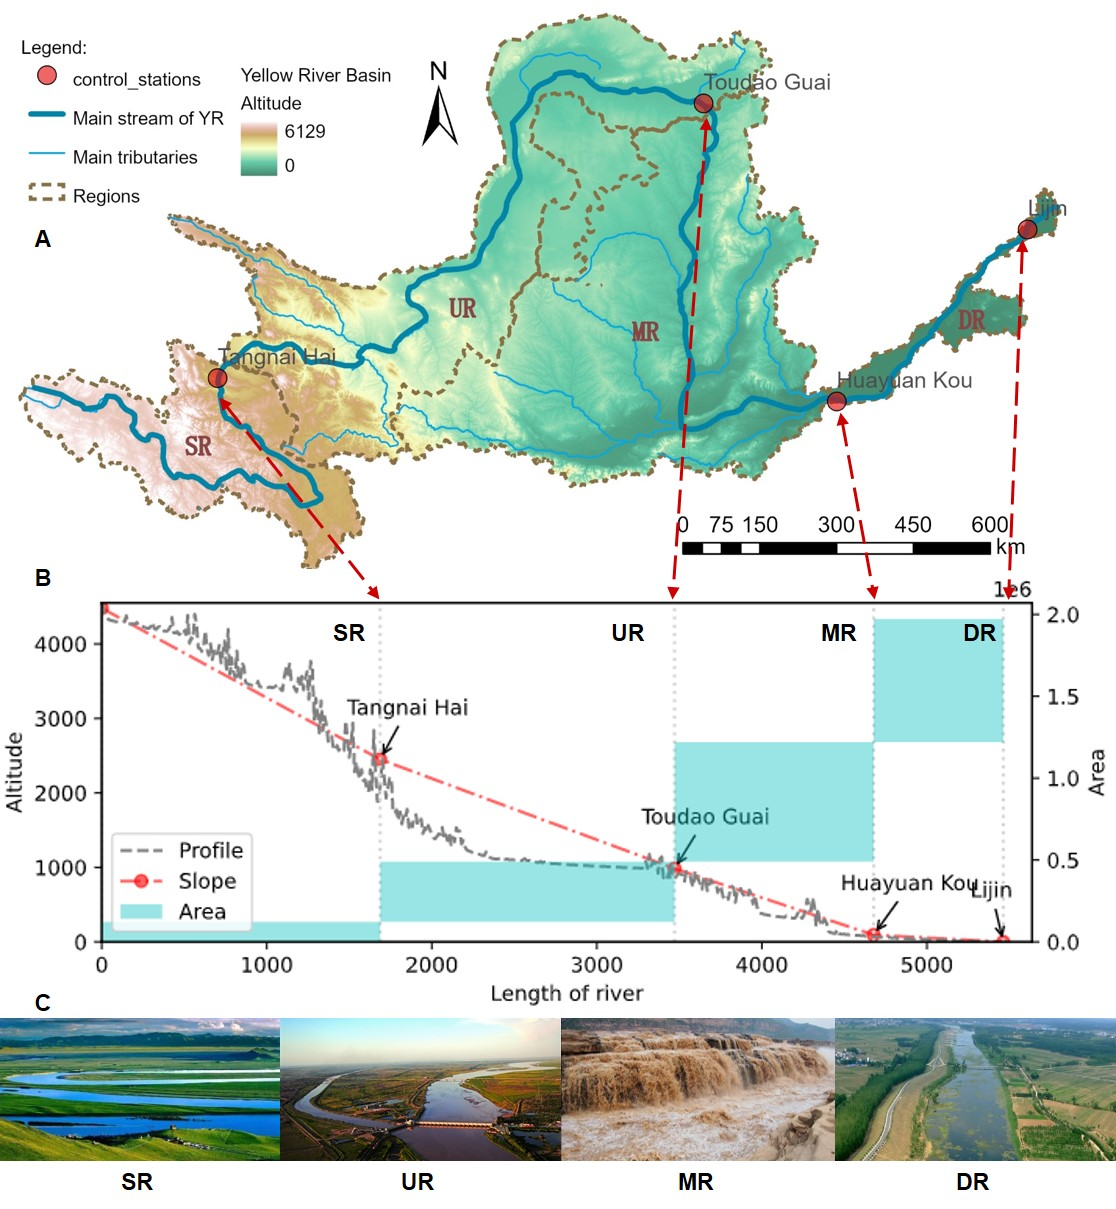
\includegraphics[width=0.8\textwidth]{../../figures/sup/s1_study_area.jpg}
    % 黄河流域示意图
    % A. 黄河流域示意图及研究区子区域的划分
    % B. 黄河主河道的剖面图
    % C. 典型景观
    \caption{
        The study area.
        \textbf{A.} Diagram of the YRB and the subdivision of the basin (SR: Source Region, UR: Upper Region, MR: Middle Region, DR: Downstream region).
        \textbf{B.} Profile of main channel of the Yellow River.
        \textbf{C.} Typical landscapes in different regions in the YRB.
    }
\end{figure}

% 补充图片2:研究区分区特征
\begin{figure}
    \centering
    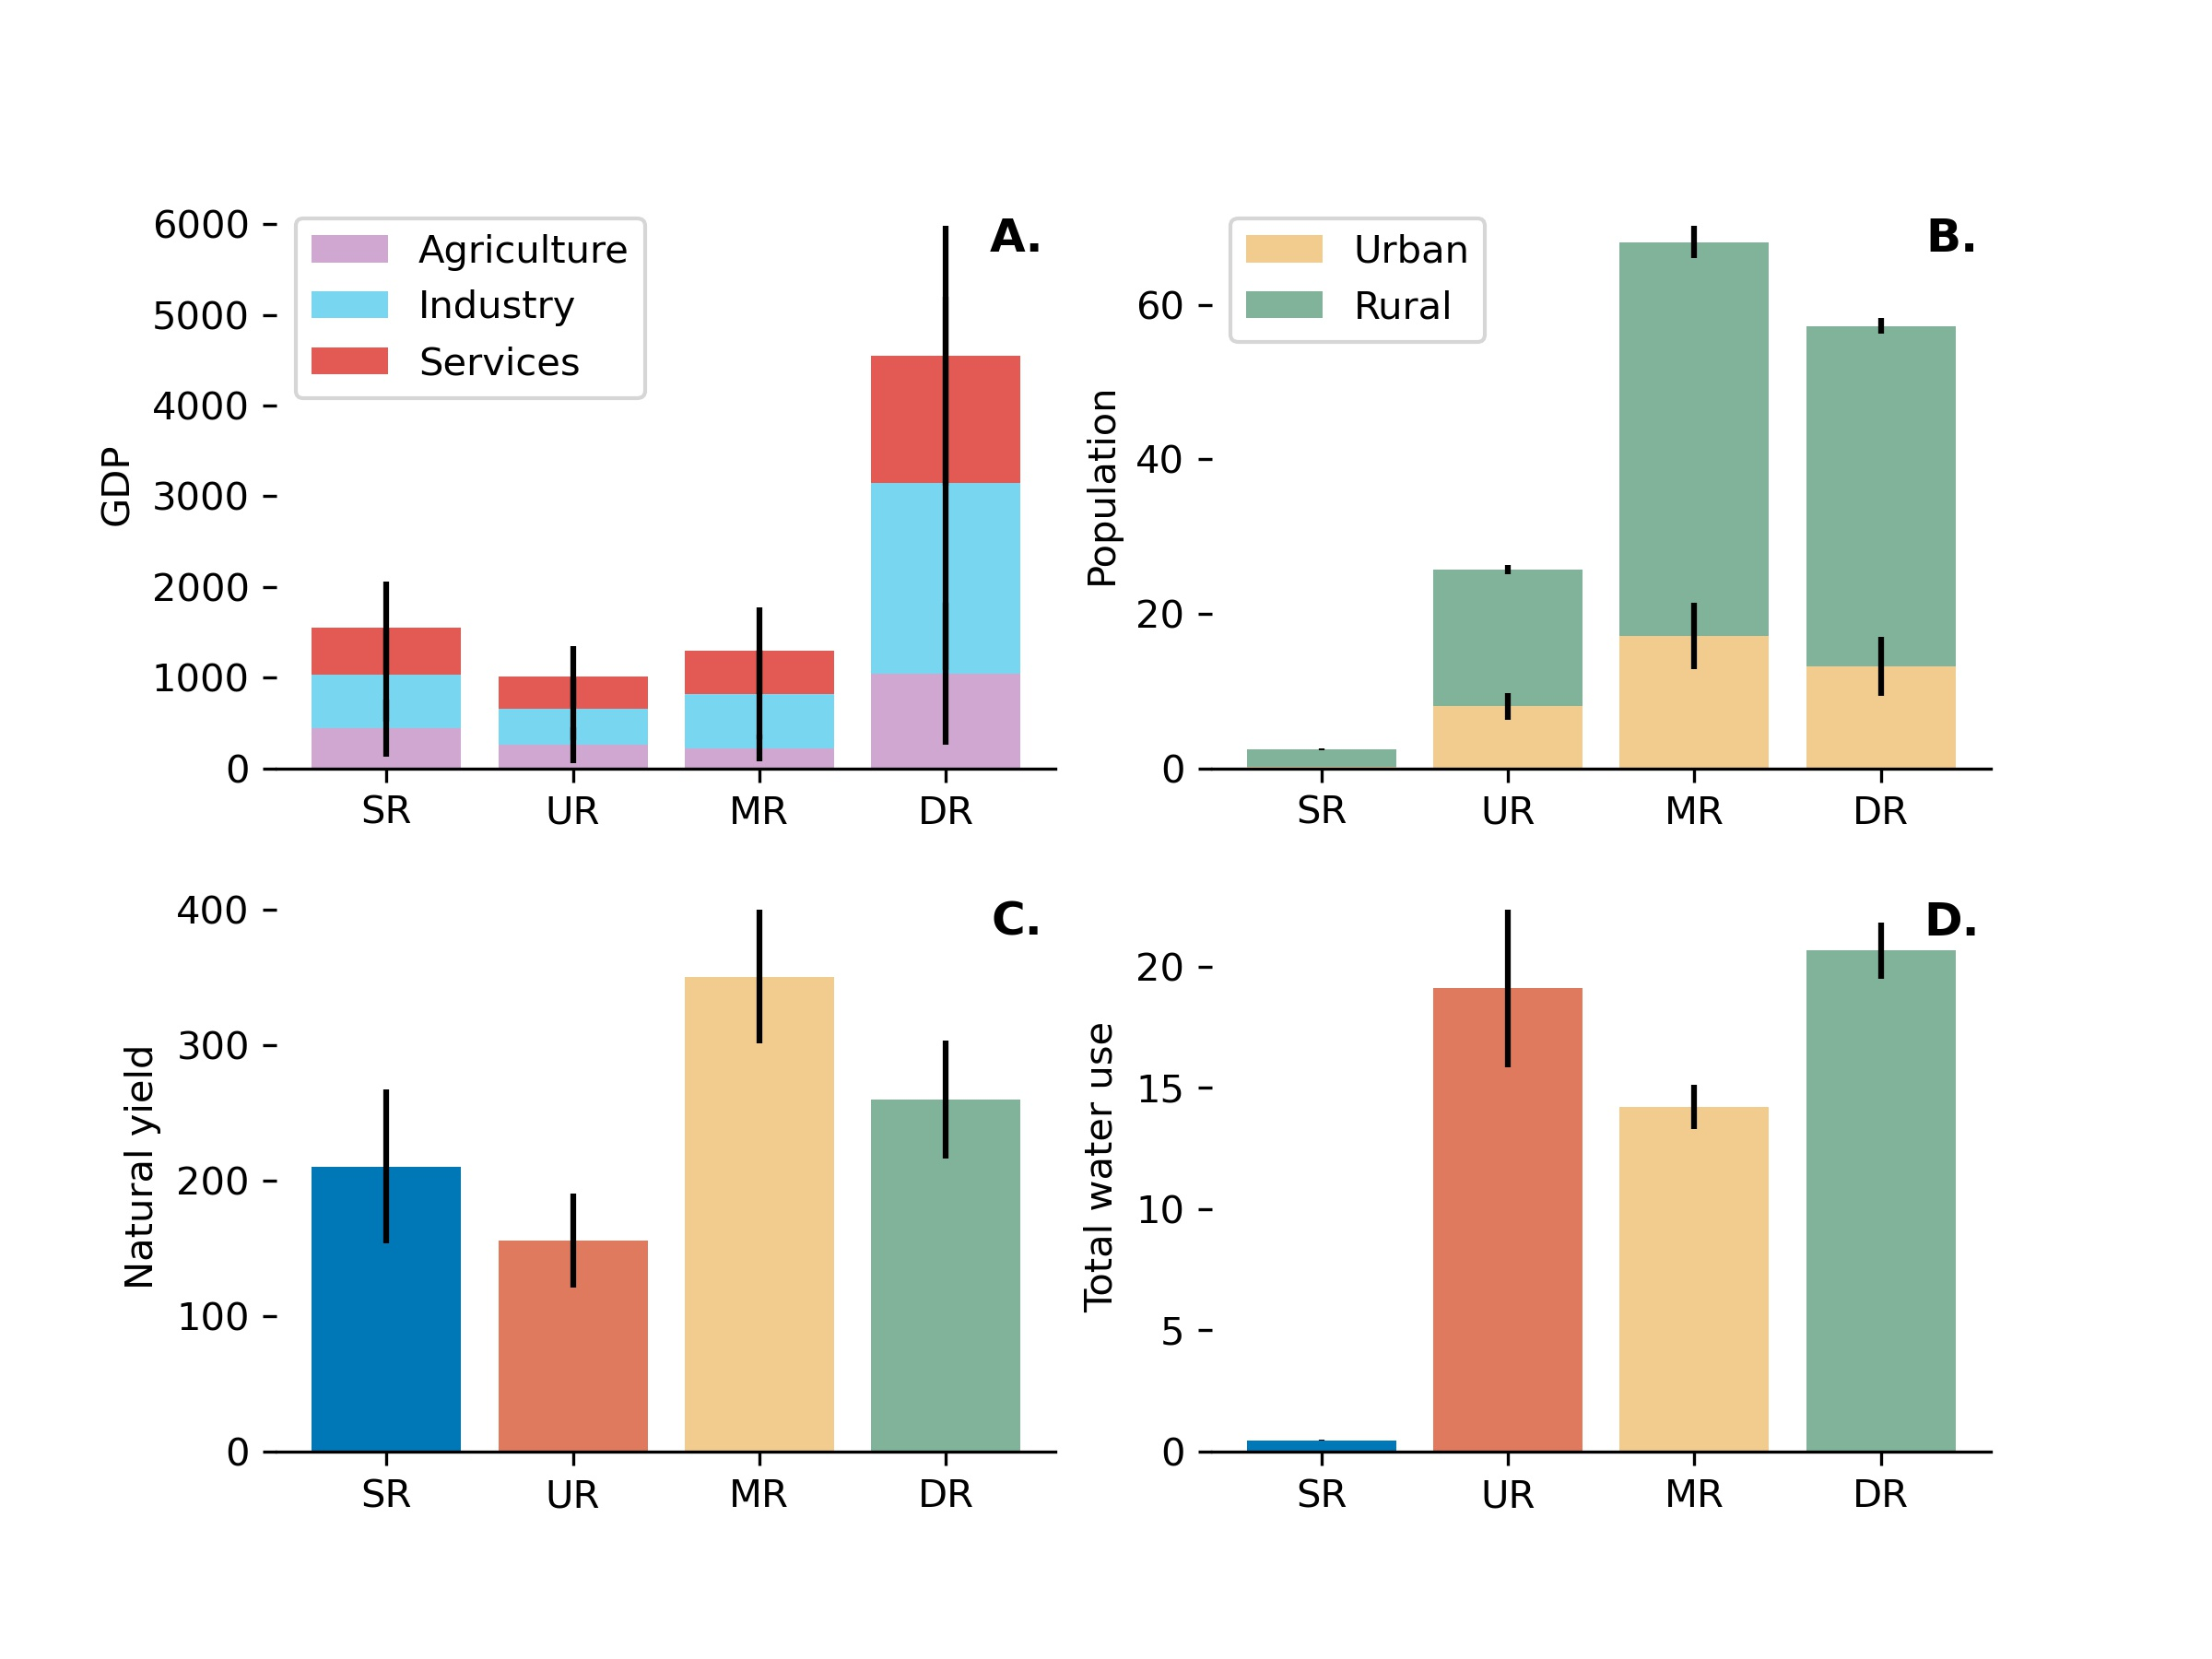
\includegraphics[width=0.8\textwidth]{../../figures/sup/region_differences.jpg}
    % 黄河流域各区域的基本社会-经济状况和水资源条件差异。
    \caption{
        Basic socio-economic status and water resource conditions of different regions in the YRB, the average from 1980 to 2000 shown.
        \textbf{A.} Proportion of GDP in different industries (primary, secondary or tertiary industry) in different regions.
        \textbf{B.} Population of urban or rural area in different regions.
        \textbf{C.} Natural water yield in different regions.
        \textbf{D.} Total water use in different regions.
    }
\end{figure}


% 补充图片3:天然水资源量
\begin{figure}
    \centering
    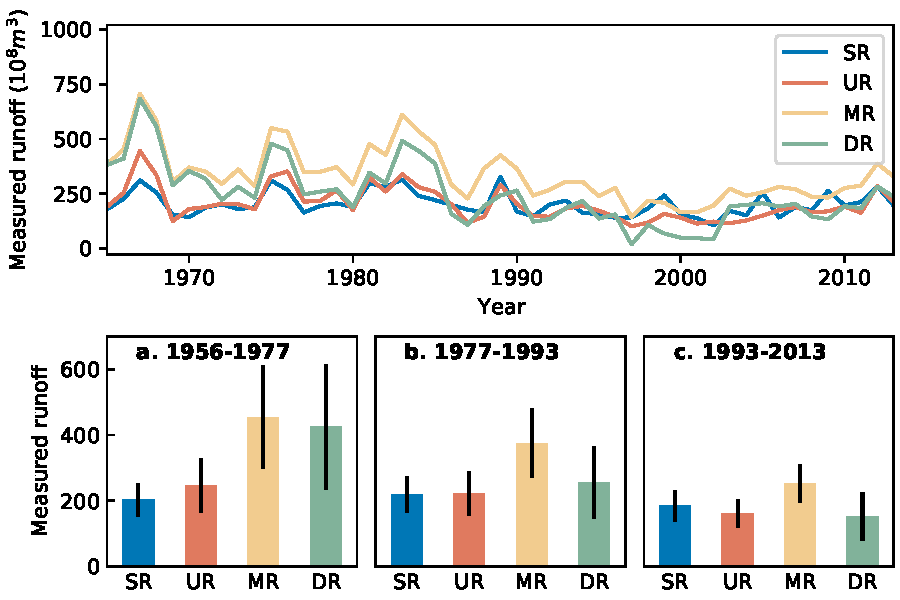
\includegraphics[width=0.8\textwidth]{../../figures/sup/sf_measured_runoff.pdf}
    \caption{Water resources in different regions. 
        \textbf{A,} changing trend of measured runoff, 
        \textbf{B, C and D} average measured runoff within different periods.
        \textbf{E, F and G} average total water consumptions within different periods. 
    }
\end{figure}


\begin{figure}
	\centering
	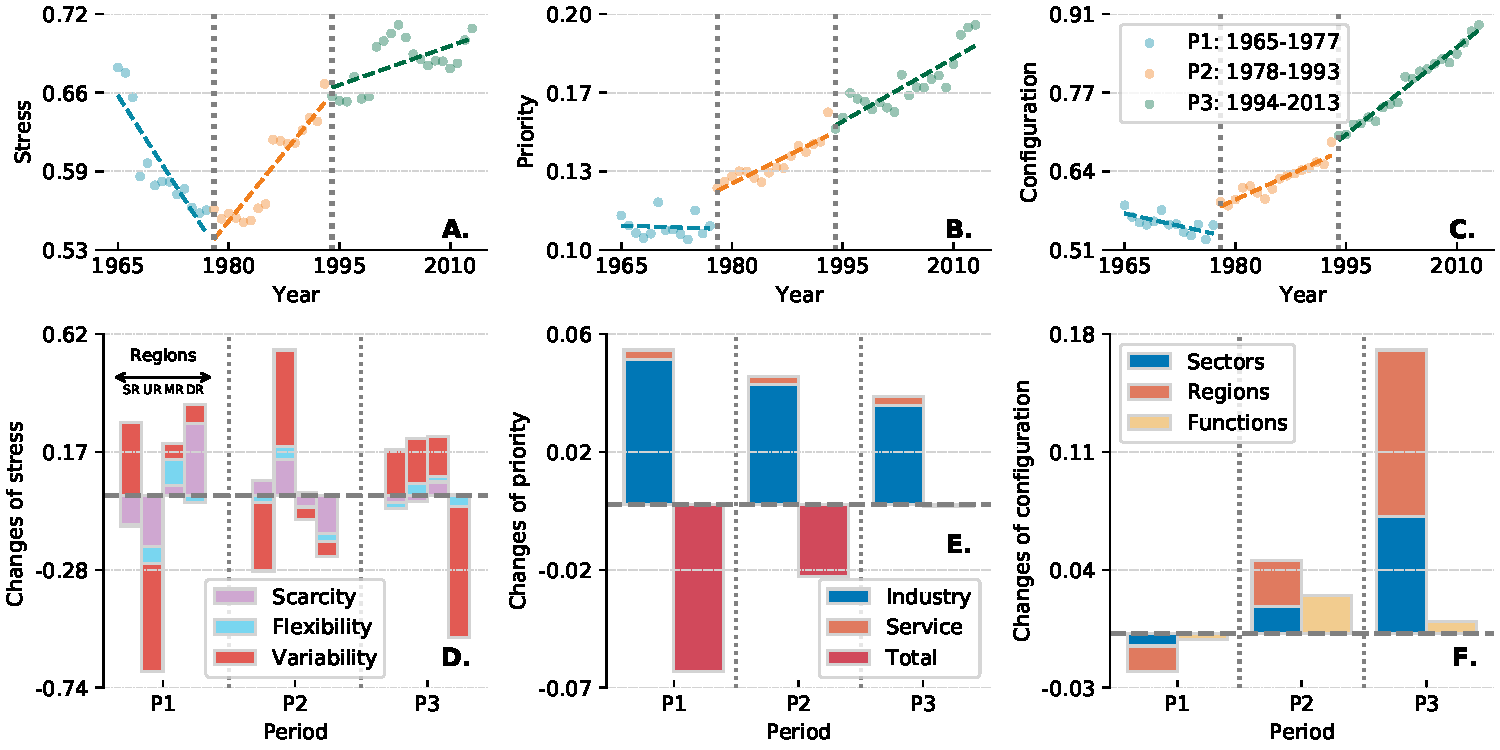
\includegraphics[width=\linewidth]{../../figures/main/dimensions.pdf}
	\caption{
		Changes in different dimensions of water resources utilization regimes and their main contributors.
		\textbf{A,} changes of water utilization stress, indicated by unstandardized scarcity-flexibility-variability water stresses index (SFV-index, see \textit{Methods} and \textit{SI Appendix} Method S4).
		\textbf{B,} changes of water utilization priority, indicated by non-provisioning water shares (see \textit{SI Appendix} Methods S4).
		\textbf{C,} changes of water utilization configuration, indicated by unstandardized distribution information entropy index (\textit{Methods} and \textit{SI Appendix} Method S4).
		\textbf{D,} Main impact factors to water utilization stresses in each period or region, and their change contributions to unstandardized SFV-index.
		\textbf{E,} Main impact water uses to water utilization priority, and their change contributions to non-provisioning water shares.
		\textbf{F,} Main impact factors to water utilization configurations, and their change contributions of related unstandardized distribution information entropy index (\textit{Methods} and \textit{SI Appendix} Method S4).
		}
	\label{fig:dimensions}
\end{figure}


% 补充图片4:水资源灵活性
\begin{figure}
    \centering
    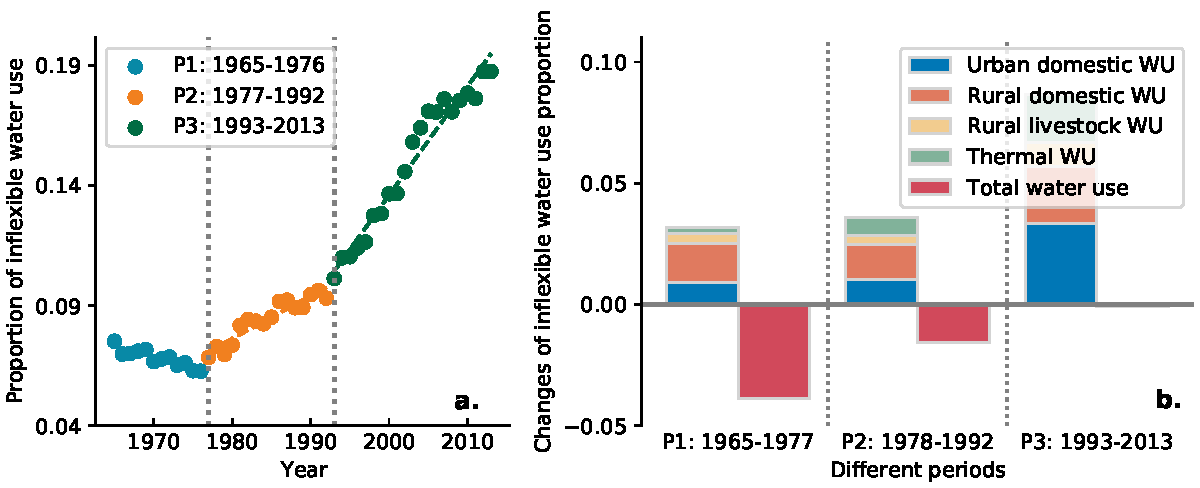
\includegraphics[width=0.95\textwidth]{../../figures/sup/inflexible_wu.pdf}
    \caption{
        Flexibility and its change contributions of water utilization.
        \textbf{A,} Proportion of inflexible water uses.
        \textbf{B,} Change contributions of inflexible water uses.
    }
\end{figure}
    

% 补充图片5:水库数量和累积库容
\begin{figure}
    \centering
    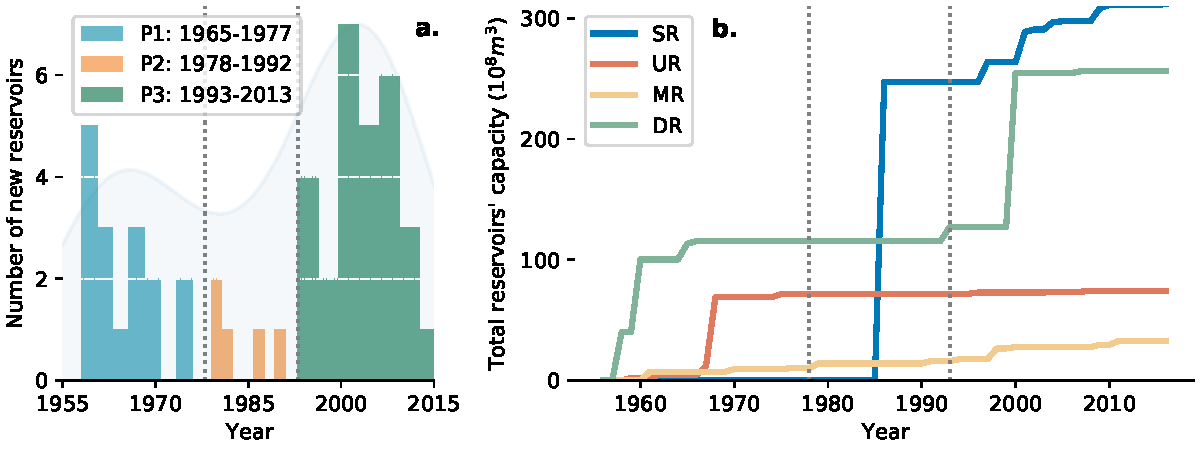
\includegraphics[width=0.95\textwidth]{../../figures/sup/reservoirs.pdf}
    \caption{
        Reservoirs and their storage.
        \textbf{A,} number of new reservoirs in different periods.
        \textbf{B,} total storage capacities in different regions. 
    }
\end{figure}

% 补充图片6:用水比例
\begin{figure}
    \centering
    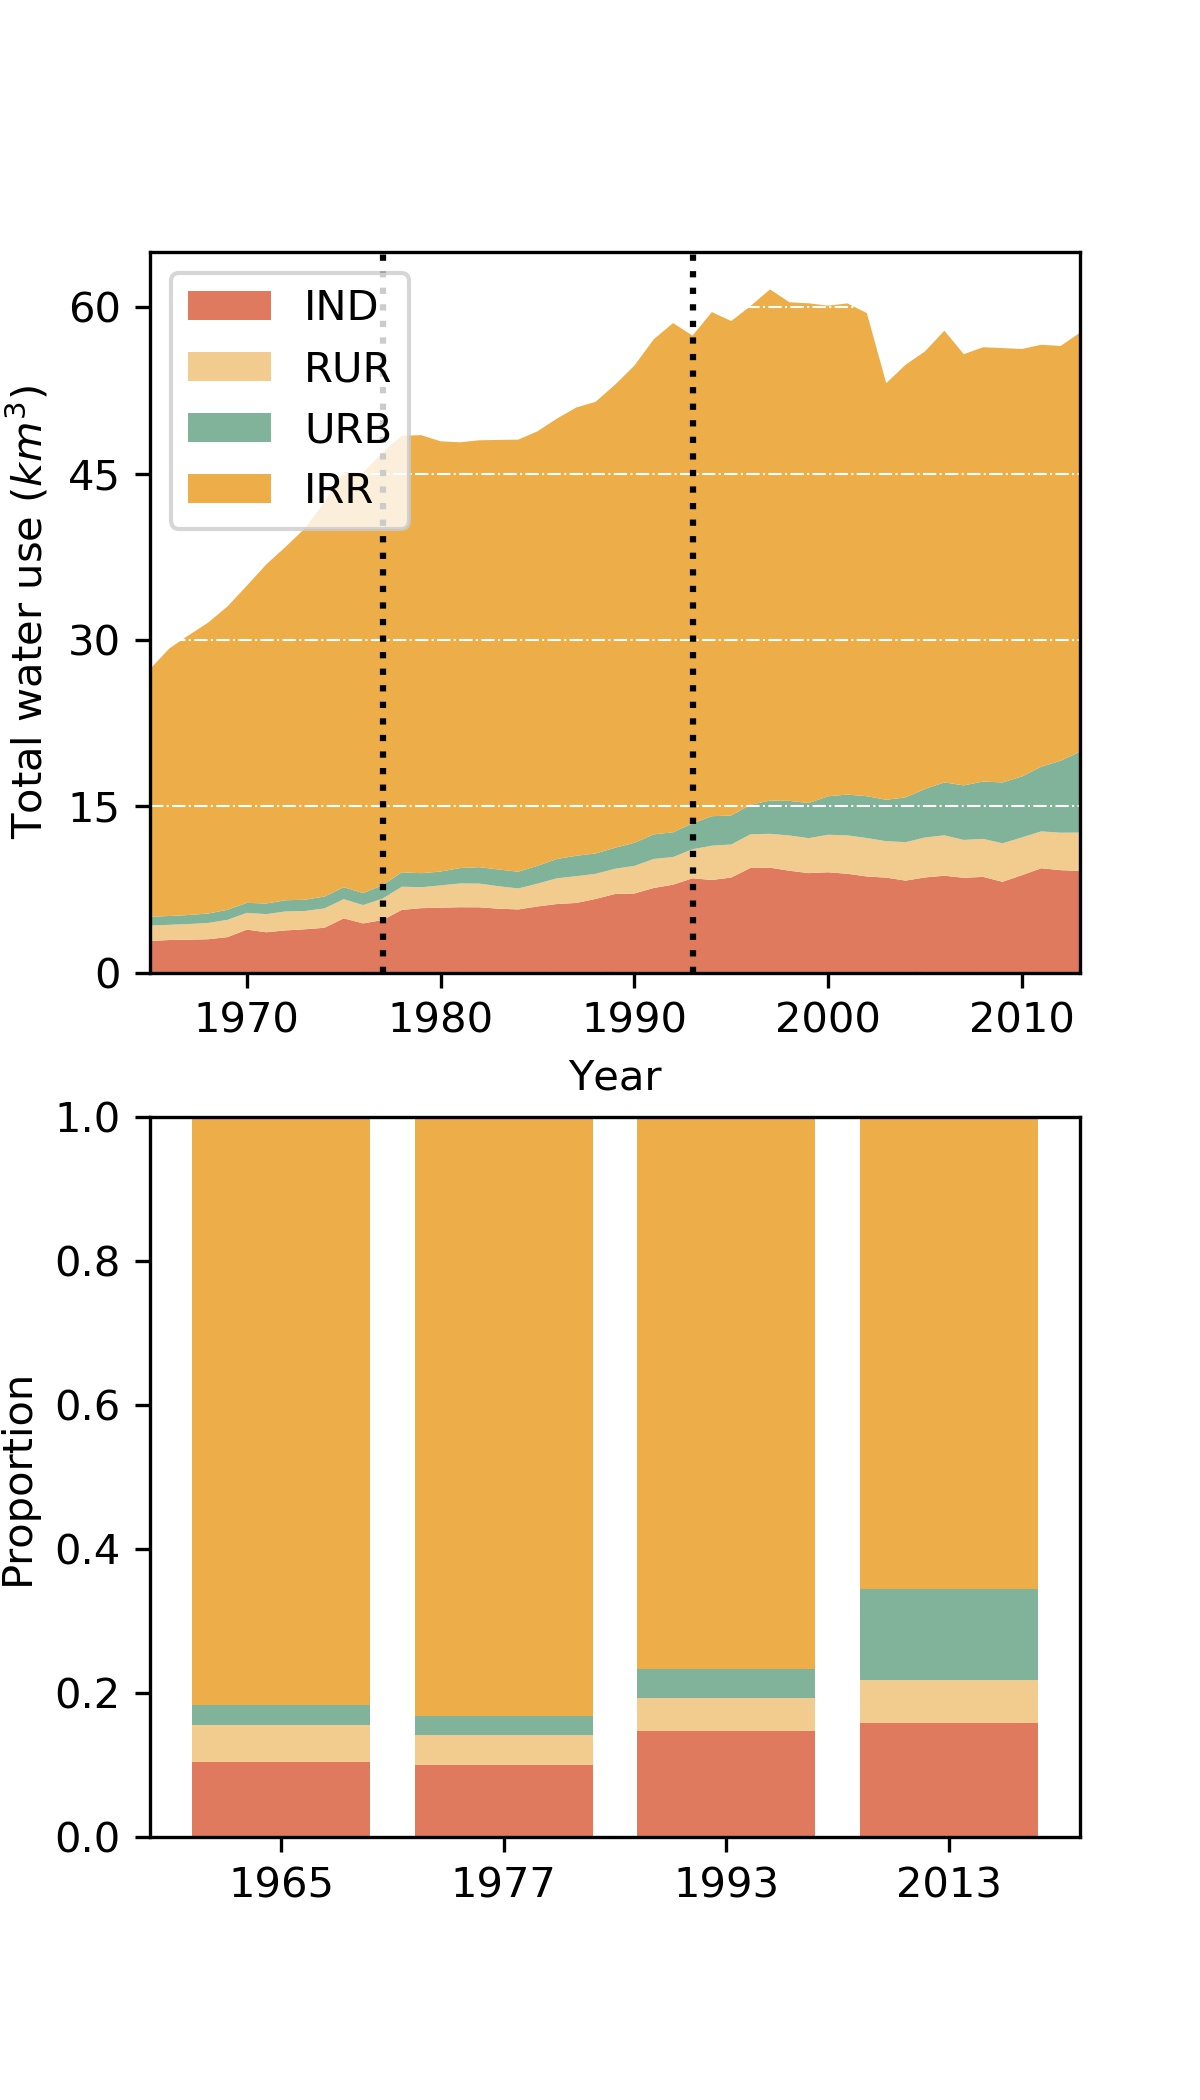
\includegraphics[width=0.6\textwidth]{../../figures/sup/sf_wu_sections_stackplot.jpg}
    \caption{Proportions of total water use between the different sectors}
\end{figure}


% 补充图片7:节水措施
\begin{figure}
    \centering
    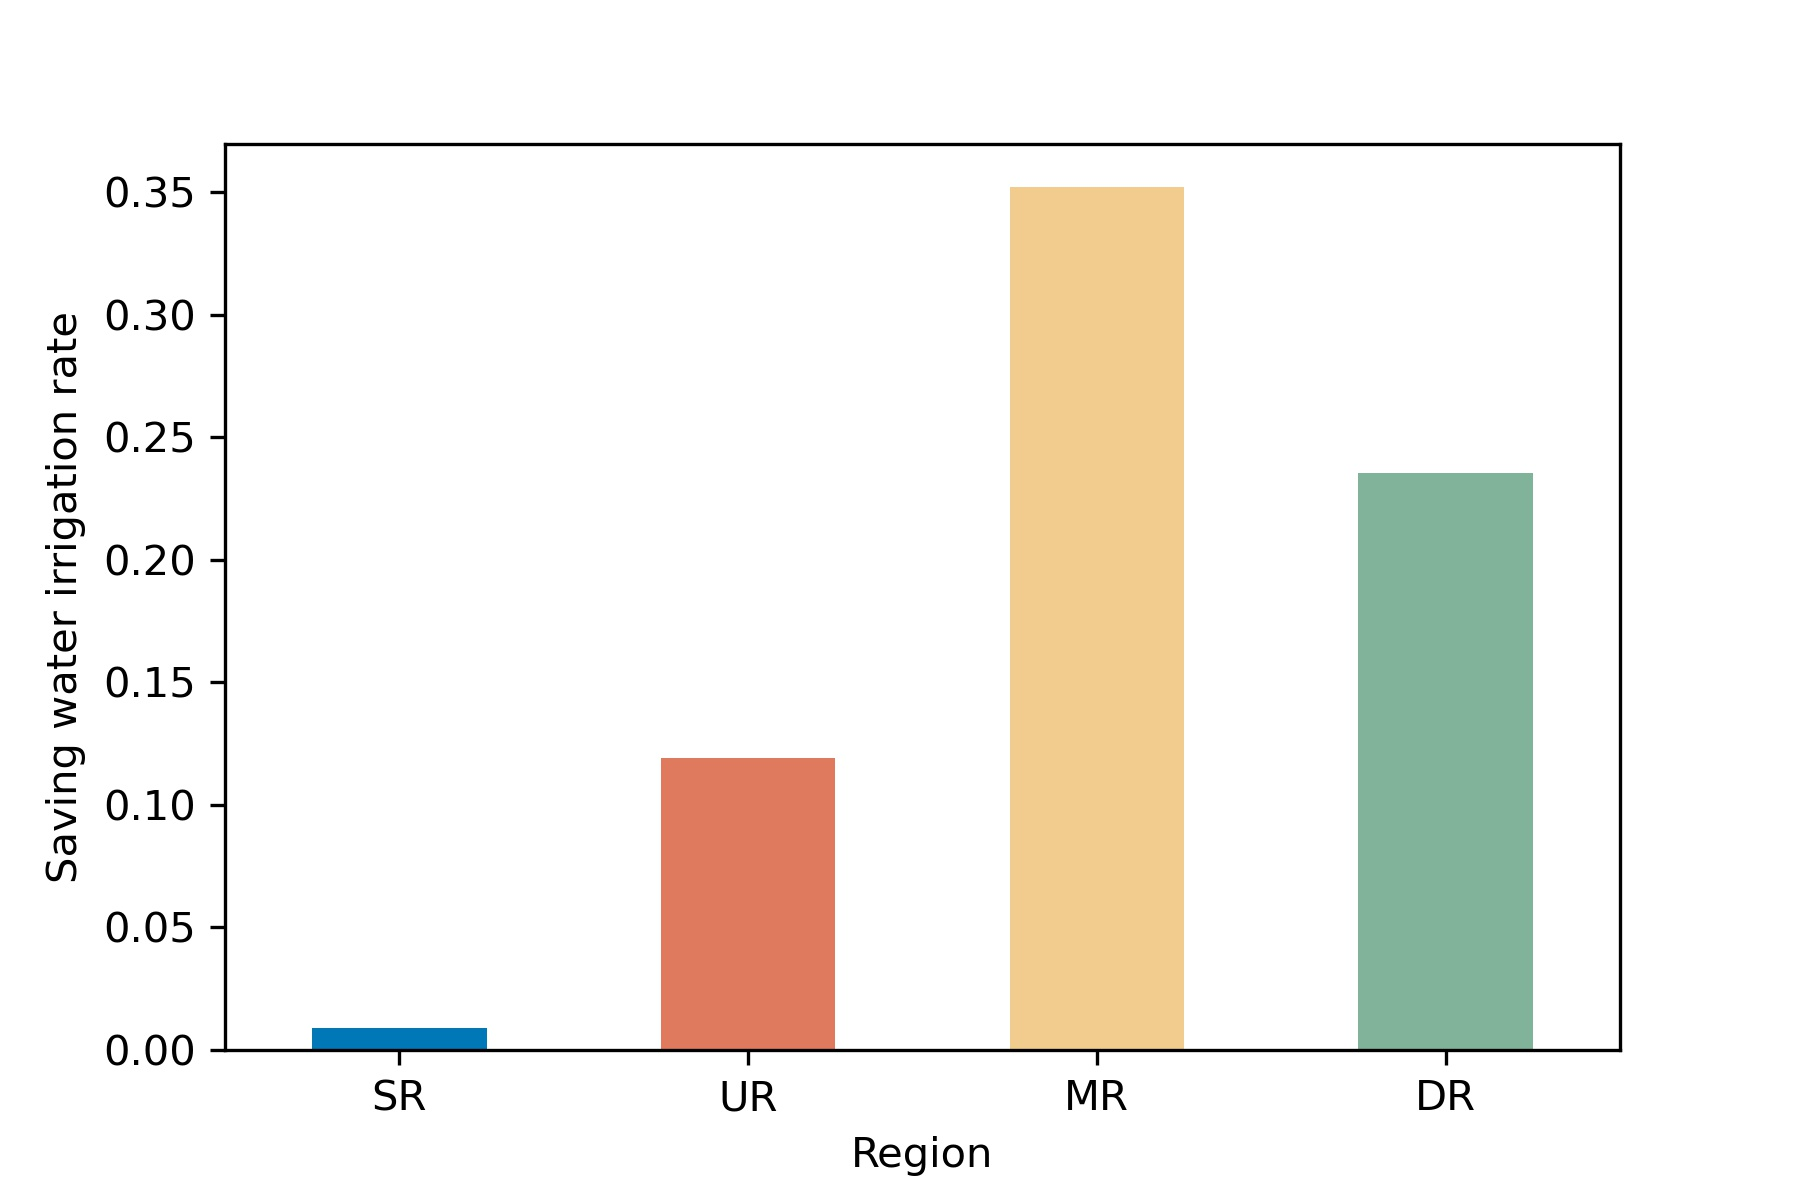
\includegraphics[width=0.6\textwidth]{../../figures/sup/saving_water.jpg}
    \caption{
        Saving water irrigated area ratio in 2013.
    }
\end{figure}


% 补充图片8:
\begin{figure}
    \centering
    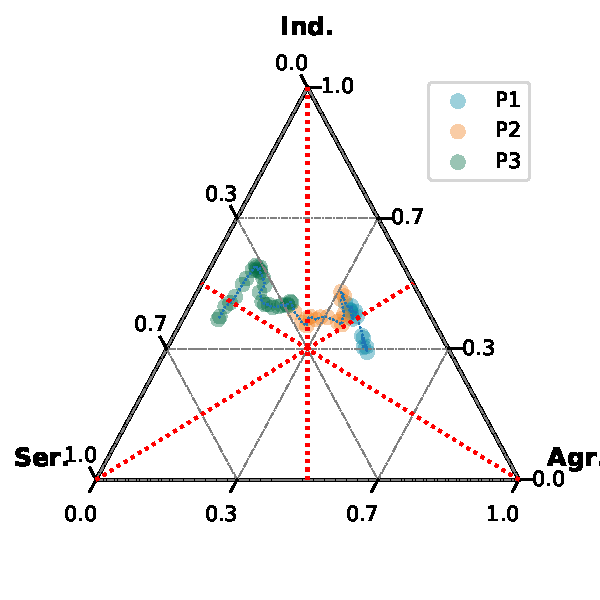
\includegraphics[width=0.5\textwidth]{../../figures/sup/ternary.pdf}
    \caption{Net contribution of agriculture, industry and services to GDP in different years.}
\end{figure}


% 补充图片9:黄河断流
\begin{figure}
    \centering
    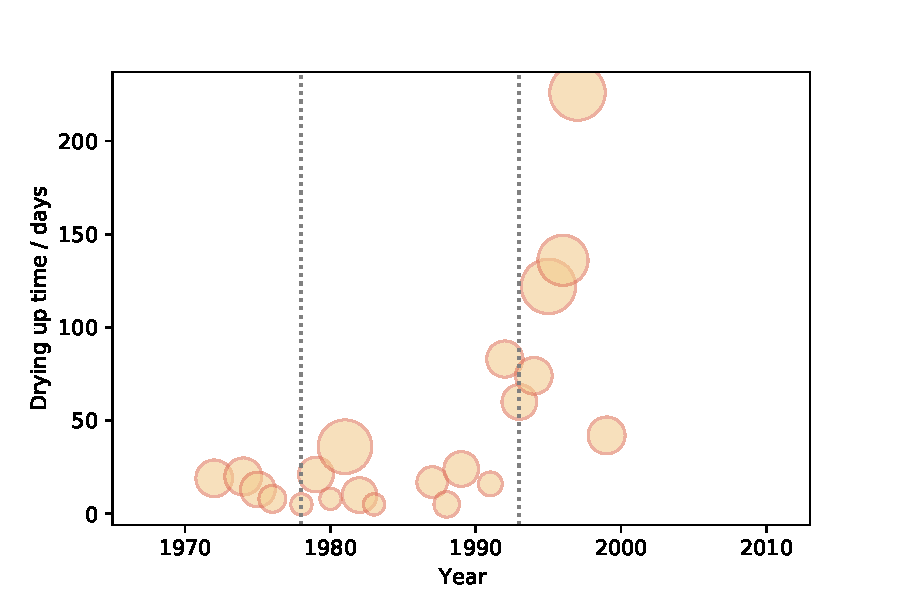
\includegraphics[width=0.6\textwidth]{../../figures/sup/outages.pdf}
    \caption{Runoff outages records, size of points indicates length of drying up river segments.}
\end{figure}

% % 补充图片10:管理政策
% \begin{figure}
%     \centering
%     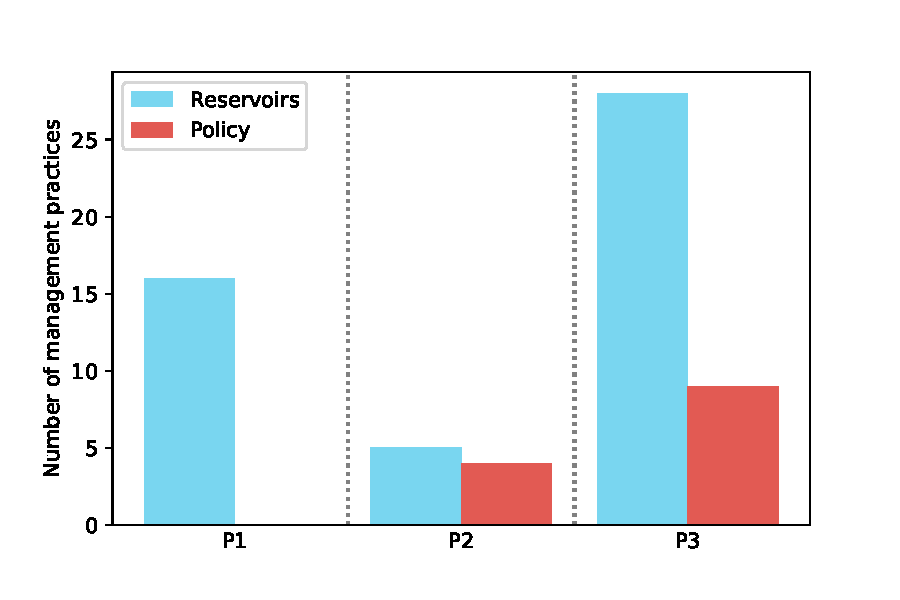
\includegraphics[width=0.95\textwidth]{../../figures/sup/managements.pdf}
%     \caption{Number of management practices in different periods, including policy and reservoirs.}
% \end{figure}

% 补充图片10:地下水
% \begin{figure}
%     \centering
%     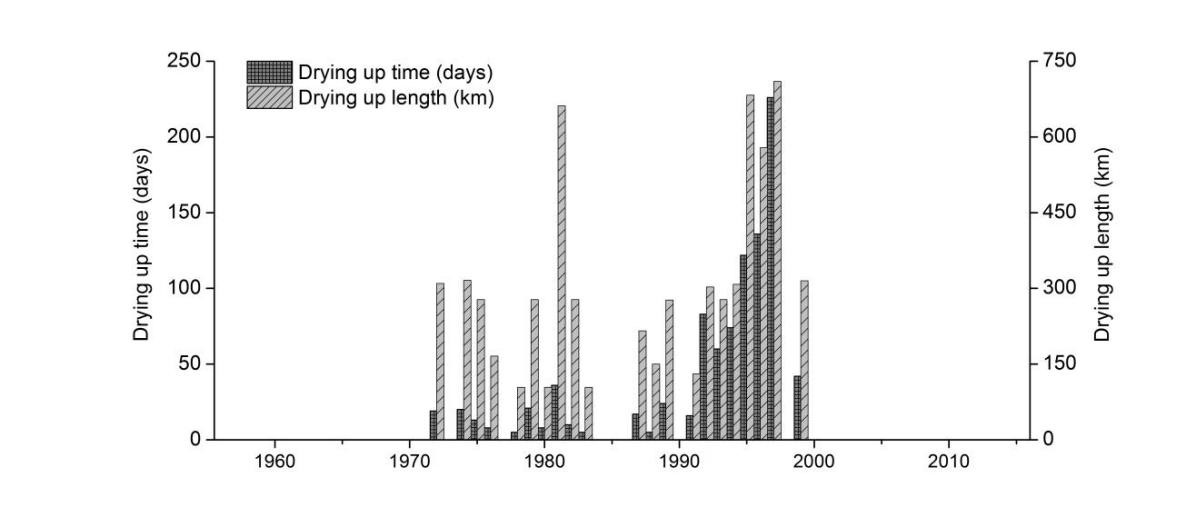
\includegraphics[width=0.95\textwidth]{../../figures/sup/outages.jpg}
%     \caption{Severe runoff outages and groundwater depletion}
% \end{figure}


% 补充图片 11 全球案例
\begin{figure}%[htbp]
	\centering
	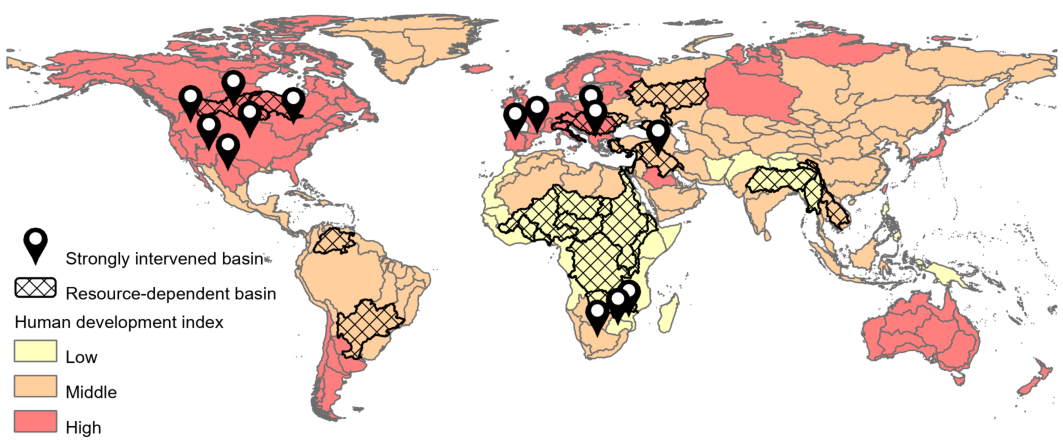
\includegraphics[width=\linewidth]{../../figures/main/map.pdf}
	\caption{
		\textbf{The Human Development Index of the world's great river basins, and the major problems facing some basins.}
		Overdependence on water resources for economic development in some basins, and high levels of human modification in others that have disrupted ecosystem structure. Data resources: Human Development Index in each basin refers from \cite{linkeGlobalHydroenvironmentalSubbasin2019}, strongly intervened basins and resource-dependent basins are come from Transboundary River Basins report by United Nations Environment Programme \url{http://geftwap.org/publications/river-basins-technical-report} \cite{unep-dhiTransboundaryRiverBasins2016}.
	}
	\label{fig:traps}
\end{figure}

补充图片10:地下水
\begin{figure}
    \centering
    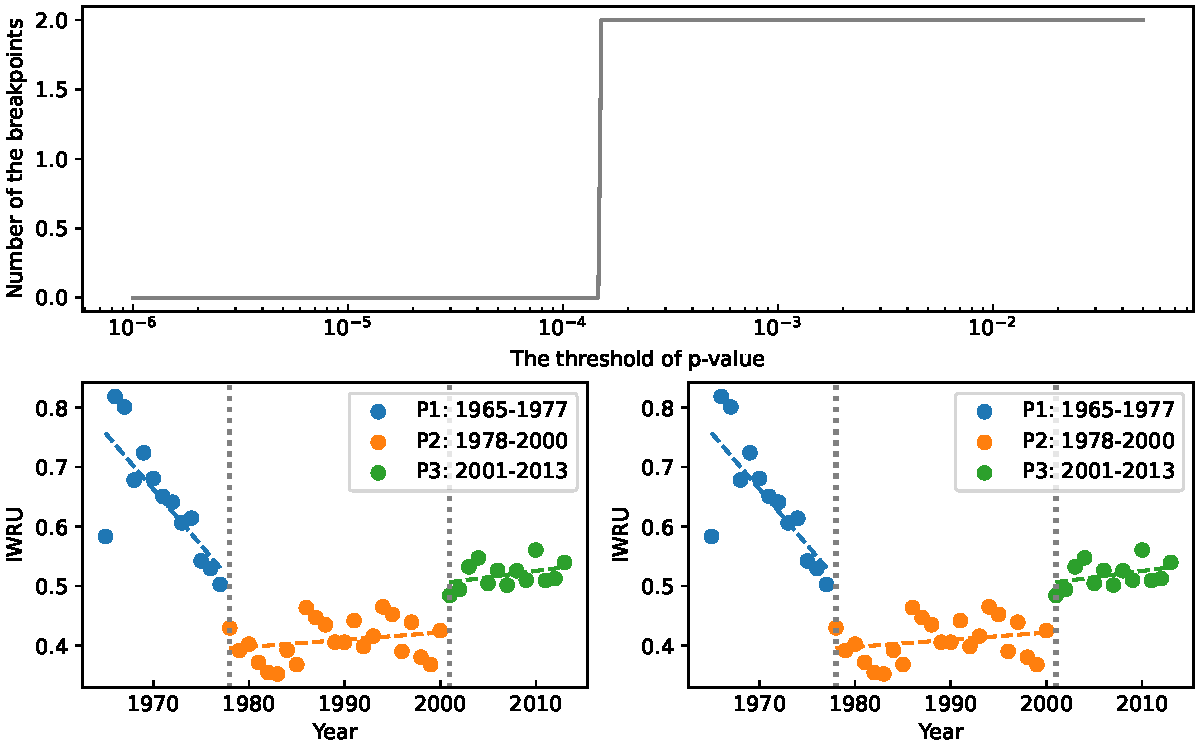
\includegraphics[width=0.95\textwidth]{../../figures/sup/sensitivity.pdf}
    \caption{
        Sensitivity analysis of the threshold of p-values. 
        \textbf{A.} number of breakpoints in different p-values.
        \textbf{B.} A typical result of two breakpoints.
        \textbf{C.} A typical result of three breakpoints.
    }
\end{figure}


%% 表格
\begin{table}\centering
    \caption{Used datasets and their sources.}
    
    % 表格
    \begin{tabular}{lrrrr}
    Dataset & Type & Spatial scale & Time limit & Source \\
    \midrule
    1. Water use & Statistical & Perfects & 1965-2013 & 2nd National Water Resources Assessment Program \\
    2. GDP & Statistical & Province & 1949-2019 & Wind database \\
    3. Groundwater and surface water use & Statistical & Watershed & 2003-2019 & Yearbooks of YRB by the YRCC. \\
    4. Reservoirs & Hydrological & Location & 1949-2015 & Wang et al. \cite{wangYellowRiverWater2019} \\
    5. Measured runoff & Hydrological & Location & 1949-2019 & Measured data from YRCC \\
    6. Laws & Political & Documents & 1949-2013 & YRCC \cite{yellowriverconservancycommissionYellowRiverBasin2013} \\
    7. History of YRCC & Political & Documents & 1949-2002 & YRCC \cite{ yellowriverarchivesOrganizationalHistoryYellow2004} \\
    \bottomrule
    \end{tabular}
\end{table}

% TODO 这里要加一个黄委会沿革的简表

%% 表格
\begin{table}\centering
    \caption{Policies and regulations above YRB level which affected the whole basin in water utilization $^a$}
    
    % 表格
    \begin{tabular}{lrr}
    Name & Year & Agency \\
    \midrule
    1. Water Law of PRC & 1988 & National People's Congress of the PRC \\
    2. Water Law of PRC -revised 1 & 2009 & National People's Congress of the PRC \\
    3. Water Law of PRC -revised 2 & 2016 & National People's Congress of the PRC \\
    4. Regulations on the Administration of Water Drawing Licences and The Collection of water resource fees & 2006 & State Council of the PRC \\
    5. Regulations on the Administration of Water Drawing Licences and The Collection of water resource fees -revised 1 & 2017 & State Council of the PRC \\
    6. Regulations on the Allocation of Water in the Yellow River & 2006 & State Council of the PRC \\
    7. Yellow River water supply distribution scheme & 1987 & State Council of the PRC \\
    8. Measures for the Administration of Water Drawing Permits & 2008 & Ministry of Water Resources of the PRC \\
    9. Measures for the Administration of Water Drawing Permits -revised 1 & 2015 & Ministry of Water Resources of the PRC \\
    10. Measures for the Administration of Water Drawing Permits -revised 2 & 2017 & Ministry of Water Resources of the PRC \\
    11. Regulations on the Allocation of Water in the Yellow River & 2006 & State Council of the PRC \\
    12. Annual distribution of available water supply of the Yellow River and main stream water dispatching scheme & 1998 & Ministry of Water Resources of the PRC \\
    13. The Yellow River water dispatching management measures & 1998 & Ministry of Water Resources \\
    14. Measures for the Implementation of the Yellow River Water Rights Conversion Management & 2004 & Ministry of Water Resources \\
    15. Regulations on the Administration of Water Drawing Licences and The Collection of water resource fees & 2006 & State Council of the PRC \\
    16. Measures for the implementation of the water drawing Permit system & 1993 \\ State Council of the PRC \\
    17. Measures for the demonstration and management of water resources in construction projects & 2002 & Ministry of Water Resources of the PRC \\
    18. Implementation Opinions on the Reform of Water Conservancy Project Management System & 2006 & State Council of the PRC \\

    \bottomrule
    \end{tabular}

    \footnotesize{$^a$ If a policy was proposed by multiple legacies, we only choose the highest one to show.}
\end{table}


%%% Add this line AFTER all your figures and tables
\FloatBarrier

% \dataset{dataset_one.txt}{Type or paste legend here.}

% \dataset{dataset_two.txt}{Type or paste legend here. Adding longer text to show what happens, to decide on alignment and/or indentations for multi-line or paragraph captions.}

\bibliography{pnas-sample}

\end{document}